%\documentclass[showpacs,preprintnumbers,amsmath,amssymb,prd]{revtex4}
%\documentclass[preprintnumbers,amsmath,amssymb,prd]{revtex4}

%\documentclass[twocolumn,showpacs,preprintnumbers,amsmath,amssymb]{revtex4}
%\documentclass[preprint,showpacs,preprintnumbers,amsmath,amssymb]{revtex4}
% Some other (several out of many) possibilities
%\documentclass[preprint,aps]{revtex4}
%\documentclass[preprint,aps,draft]{revtex4}
\documentclass[10.5pt,prb,
               showpacs,            % Pacs : showpacs, noshowpacs
               preprintnumbers,     % Preprint: preprintnumbers,
               			    %           nopreprintnumbers
               aps,                 % Society: ...
               prl,          	    % Journal Style : pra, prb, prc, prd, pre,
               			    %                 prl, prstab, rmp
               letterpaper,             % Size : a4paper, ...
               superscriptaddress,      % Affiliation (Title) : groupedaddress,
                                    %                       superscriptaddress,
                                    %                       unsortedaddress
               nofootinbib,         % Footnote: footinbib, nofootinbib
               tightenlines,        % Remove additional spaces in a line
               floats,floatfix      % Floating pictures and tables
               ,usenatbib]{revtex4-1}% Physical Review B

\usepackage{graphicx}% Include figure files
\usepackage{dcolumn}% Align table columns on decimal point
\usepackage{bm}% bold math
\usepackage{subfigure}
\usepackage{ulem}
\usepackage[table]{xcolor}
\usepackage{amsmath}
\usepackage{fancyvrb}
\usepackage[Lenny]{fncychap}
\usepackage{mathrsfs}
\usepackage{graphicx}  % needed for figures
\usepackage{dcolumn}   % needed for some tables}
%\usepackage[style=authoryear,backend=biber]{biblatex}
\usepackage{bm}        % for math
\usepackage{amsmath,amssymb}
\usepackage{hyperref}
\usepackage{color}
\definecolor{purple}{rgb}{0.58,0.0,0.83}
\usepackage{caption}
\usepackage{tabularx}
\usepackage[toc,page]{appendix}
\frenchspacing



\def\beq{\begin{equation}}
\def\eeq{\end{equation}}
\newcommand{\jav}[1]{\textcolor{red}{(jav: #1)}}

\begin{document}

\title{Cosmo Estad\'istica} 

\author{J. Alberto Vazquez}
\affiliation{ICF-UNAM}
\affiliation{CINVESTAV}
\email{javazquez@icf.unam.mx}

\author{Luis E. Padilla}
\affiliation{CINVESTAV}




\date{\today}

\begin{abstract}
 En este art\'iculo se presenta una breve introducci\'on sobre las propiedades
 que describen el Universo observable. Tanto la teor\'ia como las observaciones, y la conecci\'on existente entre
 ellas dada por la estad\'istica Bayesiana a trav\'es de c\'odigos n\'umericos. 
 \end{abstract}

%\pacs{98.65.Dx, 05.10.Cc, 95.35.+d, 98.80.Es}

\maketitle

\section{Introducci\'on}

Algo sobre el universo

%%============================================================%%
\section{El Universo observable}
%%============================================================%%


La descripci\'on est\'andar de las propiedades din\'amicas del Universo se basa en la teor\'ia 
de la Relatividad General de Einstein, la c\'ual construye una conecci\'on entre la geometr\'ia del 
espacio-tiempo y su contenido de materia a trav\'es de cantidades fundamentales, como son el 
tensor de Einstein $G_{\mu \nu}$ y el tensor de Energ\'ia-momento $T_{\mu \nu}$
%
	\beq  \label{eq:Ricci}
		G_{\mu \nu} \equiv R_{\mu \nu} - \frac{1}{2}g_{\mu \nu}R =  8\pi G T_{\mu \nu}.
	\eeq
 
 \noindent
La parte izquierda de la igualdad describe la geometr\'ia del espacio-tiempo englobada en las 
componentes del tensor de Ricci $R_{\mu \nu}$, el escalar de Ricci $R$ y la m\'etrica del espacio-tiempo
$g_{\mu \nu}$. \'Estas en conjunto dirigen el comportamiento de los constituyentes $T_{\mu \nu}$ del Universo.
Una modificaci\'on aceptable a las ecuaciones de Einstein es la introducci\'on de una  invariante
bajo transformaciones de Lorentz $\Lambda g_{\mu \nu}$ en las ecuaciones de campo
%
	\beq \label{eq:Einstein}
		R_{\mu \nu} - \frac{1}{2}g_{\mu \nu}R + \Lambda g_{\mu \nu}=  8\pi G T_{\mu \nu},
	\eeq
%
donde $\Lambda$ es la denominada constante cosmol\'ogica y su valor, de acuerdo con observaciones astrof\'isicas,
es $\Lambda \sim10^{-52} m^{-2}$; veremos un poco m\'as acerca de esta componente en la siguiente secci\'on.
El sistema de ecuaciones (\ref{eq:Einstein}) son, en general, un conjunto de ecuaciones diferenciales parciales acopladas 
cuasi-lineares y de segundo orden para los diez elementos del tensor m\'etrico. Sin embargo, \'estas pueden 
presentar soluciones anal\'iticas simples en la presencia de simetr\'ias gen\'ericas, como veremos a continuaci\'on.



%%============================================================%%
\section{Geometr\'ia del espacio-tiempo}
%%============================================================%%


Para poder especificar la geometr\'ia del Universo, una suposici\'on escencial es el \textit{Principio Cosmol\'ogico}:
a escalas suficientemente grandes, a un tiempo particular, el Universo observable 
puede considerarse como \textit{Homog\'eneo e Isotr\'opico} con gran precisi\'on.
Por ejemplo, en escalas superiores a $100$ Mega-parsecs\footnote[1]{1 parsec (pc) $\simeq 3.261$ a\~nos luz} 
la distribuci\'on de galaxias observadas sobre la esfera celeste justifica la suposici\'on de isotrop\'ia. 
%
Adem\'as de esto, la uniformidad
observada en la distribuci\'on de temperaturas [una parte en $10^5$] medida a trav\'es de la radiaci\'on C\'osmica en el Fondo de
Microondas (CMB) es la mejor evidencia observacional que tenemos a favor de una 
isotrop\'ia universal. Por tanto, s\'i la isotrop\'ia se da por sentado y teniendo en cuenta que nuestra
posici\'on ocupada en el Universo no tiene preferencia sobre ninguna otra -conocido como el \textit{Principio 
Copernicano}- por tanto la homogeneidad se sigue de considerar isotrop\'ia en cada punto.
 \\
 
 	\fbox{
	 	\parbox[c][1.cm][c]{0.95\textwidth\linespread{1.5}\selectfont{}}
			{
			\textbf{Homogeneidad} establece que el Universo se observa por igual en cada punto del espacio. \par
			\textbf{Isotrop\'ia} establece que el Universo se observa por igual en todas las direcciones.
			}
		}
	\vspace{1em}


%%------------------------------------------------------------------------------------------------%%
\subsection*{M\'etrica Friedmann-Robertson-Walker}
%%------------------------------------------------------------------------------------------------%%



Vamos a incorporar los postulados de Homogeneidad e Isotrop\'ia en la descripci\'on geom\'etrica del Universo. 
El primero demanda que todos lo puntos sobre una hiper-superficie espacial sean equivalentes,
mientras que el segundo asegura que todas las direcciones sobre dicha hiper-superficie tambi\'en son 
equivalentes para observadores fundamentales. Esto es, isotrop\'ia requiere que la distribuci\'on 
de galaxias a dos tiempos distintos sea similar, mientras que la homogeneidad requiere
que el factor de magnificaci\'on deba ser independiente de la posici\'on de la distribuci\'on. 
%
Adem\'as, a trav\'es de los a\~nos, observaciones cosmol\'ogicas han dado evidencia contundente de  que 
el Universo actual se encuentra en un per\'iodo de expansi\'on. 
%y por tanto el factor de escala satisface 
%la condici\'on $\dot a(t)>0$.
%
De esta manera es preciso describir nuestro Universo con una m\'etrica que contenga toda esta informaci\'on.  
\'Esta m\'etrica que describe las escalas m\'as grandes se le conoce
como m\'etrica de Friedmann-Robertson-Walker (FRW), y esta dada por el siguiente intervalo
%Por otro lado, el tensor $\gamma_{ij}$ contiene solo funciones dependientes de las coordenadas.
%Adem\'as, el espacio-tiempo que cumple con las propiedades de homogeneidad e isotr\'opia es aquel
%cuyas propiedades quedan especificadas con tan solo una constante - la \textit{curvatura} $K$.
%Este tipo de espacios, denominados {\it maximalmente sim\'etricos}, definen la parte espacial de la m\'etrica
%como
%
%	\beq \label{eq:FRW2}
%		\gamma_{ij} dx^i dx^j = \frac{dr^2}{1- Kr^2} + r^2d\Omega^2,
%	\eeq
%
%donde $r$ es la coordenada radial y $d\Omega^2 = d\theta^2 + \sin^2 \theta d\phi^2$ es la m\'etrica de la 2-esfera.
%Por tanto, sustituyendo (\ref{eq:FRW2}) en (\ref{eq:FRW}), la m\'etrica FRW se reescribe de la siguiente forma

	\beq \label{eq:FRW3}
		ds^2 = dt^2 - a^2(t)\left[\frac{dr^2}{1-Kr^2} + r^2d\Omega^2 \right].
	\eeq
%
donde $r$ es la coordenada radial y $d\Omega^2 = d\theta^2 + \sin^2 \theta d\phi^2$ es la m\'etrica de la 2-esfera. 
Al t\'ermino $a(t)$ se le conoce como el factor de escala normalizado y representa la funci\'on 
de magnificaci\'on de nuestro Universo. N\'otese que para obtener un Universo en expansi\'on 
es necesario que $\frac{d a(t)}{dt}>0$. La constante $K$ describe la geometr\'ia de las secciones espaciales 
y dependiendo del valor $K>0,~ K=0$ o $K<0$
representa Universos tipo cerrado $\mathcal{S}^3$, plano $\mathcal{R}^3$ o abierto $\mathcal{H}^3$  respectivamente.
%
Considerando la m\'etrica $g_{\mu \nu}$ de la forma (\ref{eq:FRW3}), los \'unicos t\'erminos de curvatura distintos de cero son
%
	\begin{eqnarray} \label{eq:R_FRW}
		R^0_0 &=& -\frac{3\ddot a}{a},\label{eq:curvs1}  \qquad
		R^i_j = \left(\frac{\ddot a}{a}+\frac{2\dot a^2}{a^2} +
				  \frac{2\kappa}{a^2} \right)\delta^i_j, \label{eq:R2} \qquad
		R     = 6 \left(\frac{\ddot a}{a} +\frac{\dot a^2}{a^2}+ 
				  \frac{\kappa}{a^2} \right). \label{eq:R3}
	\end{eqnarray}

o,  a partir de (\ref{eq:Ricci}) y (\ref{eq:R_FRW}), el tensor de Einstein esta dado por

	\begin{equation}
		G^0_0 = 3 \left[ \left( \frac{\dot a}{a} \right)^2 + \frac{K}{a^2} \right], \qquad 
				G^i_j =\left[2\frac{\ddot a}{a} + \left( \frac{\dot a}{a} \right)^2  + \frac{K}{a^2}\right]\delta^i_j.
	\end{equation}

Por tanto, la din\'amica del espacio-tiempo en un universo homog\'eneo e isotr\'opico se reduce a determinar
el factor de escala normalizado $a(t)$, el cual se calcula una vez que el contenido de materia queda especificado.


%%============================================================%%
\section{Inventario C\'osmico}
%%============================================================%%


Una vez que se ha especificado la geomtetr\'ia del espacio-tiempo solo falta definir el contenido de materia  
para resolver las ecuaciones de Einstein. 
Consideraremos a los \textit{fluidos perfectos} ideales como la principal fuente del tensor
de energ\'ia-momento
%
	\beq
		T^{\mu \nu} = (\rho + p)u^\mu u^\nu - p g^{\mu \nu},
	\eeq
%
donde $\rho$ es la densidad de energ\'ia y $p$ es la presi\'on isotr\'opica del fluido, ambas
medidas por un observador en el sistema de referencia inercial local, en el cual el fluido
se encuentra en reposo. En \'este sistema, donde la 4-velocidad del fluido es $u^{\mu}=(1,0,0,0)$,
el tensor de energ\'ia-momento se reduce a $T^{\mu}_\nu=diag(-\rho, g^{ii}p)$. 
%
La componente $00$ de Einstein nos proporciona la ecuaci\'on de Friedmann
%
	\beq \label{eq:Fried}
		\left(\frac{\dot a}{a}\right)^2 = \frac{8\pi G}{3} \rho - \frac{k}{a^2} + \frac{\Lambda}{3}.
	\eeq


Por otro lado, dado $T^{\mu}_\nu$ se puede obtener la conservaci\'on de la energ\'ia a partir de $\nabla_\mu T^\mu_\nu=0$,
la cual conlleva a la ecuaci\'on de continuidad
%
	\beq \label{eq:conti}
		\dot \rho + 3 \frac{\dot a }{a}(\rho + p) = 0.
	\eeq 

\noindent
Para poder entender las propiedades din\'amicas del Universo, primero se necesita tener en cuenta
el contenido total de \'este. Nuestro enfoque se basa en los fluidos perfectos barotr\'opicos que satisfacen 
una {\it ecuaci\'on de estado} dependiente del tiempo $w(a)$ de la forma $p = w(a)\rho,$
para cualquier componente. Si adem\'as se considera $w$ igual a una constante, la ecuaci\'on de continuidad (\ref{eq:conti})
puede ser integrada f\'acilmente para obtener
%
	\beq 
		\rho \propto a^{-3(1+w)}.
	\eeq

\noindent
Adem\'as, en un Universo dominado por la densidad de energ\'ia $\rho$ la 
ecuaci\'on de Friedmann (\ref{eq:Fried}) nos lleva a la evoluci\'on temporal del factor de escala
%
	\beq
		a \propto t^{2/3(1+w)}, \qquad  w\neq -1.
	\eeq

\noindent
Esto es, la evoluci\'on del Universo cuya \'unica componente es un fluido perfecto puede calcularse una 
vez especificada su ecuaci\'on de estado. El modelo de materia oscura fr\'ia con constante
cosmol\'ogica ($\Lambda$CDM) se basa en cuatro ingredientes principales descritos por: la 
radiaci\'on (fot\'ones y neutrinos sin masa), materia en forma de bariones y una contribuyente de materia
oscura fr\'ia (DM) y la energ\'ia del vac\'io $\Lambda$. El comportamiento de cada uno de estos
constituyentes se resume de la siguiente manera:



%%------------------------------------------------------------------------------------------------%%
\subsection*{Radiaci\'on}
%%------------------------------------------------------------------------------------------------%%


Esta componente relativista domina durante las etapas tempranas del Universo y 
se caracteriza por tener una presi\'on asociada $p_r=\rho_r/3$, y por tanto una ecuaci\'on de estado 
$w_r=1/3$. Adem\'as la evoluci\'on de la densidad de energ\'ia y el factor de escala est\'an dados por 
%
	\beq
		\rho_r(t) \propto a^{-4}, \qquad {\rm and} \qquad a(t)\propto t^{1/2}.
	\eeq
	
\noindent
La densidad de energ\'ia de la radiaci\'on total en el Universo puede describirse en t\'erminos
de dos contribuyentes principales: fotones ($\gamma$) y neutrinos sin masa ($\nu$):
%
	\beq
		\rho_r = \rho_\gamma(t) + \rho_\nu(t).
	\eeq

\textit{Fotones}. Los fotones primordiales juegan un papel muy importante en la cosmolog\'ia 
observacional  ya que ellos constituyen la radiaci\'on c\'osmica en el fondo de microondas que observamos
hoy en d\'ia \jav{ \cite{alguna cita}}
\\

\textit{Neutrinos sin masa}. Los neutrinos son clasificados como leptones d\'ebilmente interactuantes los cuales existen
en tres sabores: electr\'on $\nu_e$, muon $\nu_\mu$ y tau $\nu_\tau$; todos ellos tienen asociado una antipart\'icula. 
La densidad de energ\'ia  de los neutrinos que permea el cosmos (estimada a partir de argumentos te\'oricos) esta
dada por 
%
	\beq \label{eq:nu}
		\rho_\nu = N_{\rm eff} \times \frac{7}{8}\times \left(\frac{4}{11} \right)^{4/3}\rho_\gamma,
	\eeq

\noindent
donde $N_{\rm eff}$ es el n\'umero efectivo de especies de neutrinos; n\'otese que considerando el modelo est\'andar se tiene $N_{\rm eff}=3.046$.
Recientemente varios experimentos sugieren que los neutrinos efectivamente poseen 
una masa aunque muy peque\~na, por ejemplo experimentos que detectan neutrinos atmosf\'ericos o neutrinos solares.
Aunado a esto, obervaciones cosmol\'ogicas tambi\'en pueden imponer l\'imites en las masas de los neutrinos; algunos art\'iculos
de revisi\'on sobre el tema \jav{\cite{algo}}.


%%------------------------------------------------------------------------------------------------%%
\subsection*{Materia}
%%------------------------------------------------------------------------------------------------%%

Cualquier tipo de material con presi\'on despreciable es usualmente considerada como \textit{polvo}. 
Esta propiedad se representa a trav\'es de una ecuaci\'on de estado $w_m=0$ y densidad de energ\'ia dada por
%
	\beq
		\rho_m(t) \propto a^{-3}, \qquad {\rm} \qquad a(t)\propto t^{2/3}.
	\eeq
	
\noindent
El contenido total de materia del universo viene en diferentes formas,  por ejemplo, adem\'as de la materia bari\'onica que 
com\'unmente conocemos y observamos en el laboratorio, observaciones en la estructura del Universo a gran escala 
sugieren que la mayor cantidad del contenido gal\'actico es de la forma de alg\'un tipo no-bari\'onico de materia, denominada 
como \textit{materia oscura}. 
La densidad de materia total puede expresarse como la suma de las contribuciones bari\'onicas (b)
y de materia oscura (DM)
%
	\beq
		\rho_m(t) = \rho_{\rm b}(t) + \rho_{DM}(t).
	\eeq

\textit{Bariones}. Son las bases de la materia que f\'acilmente localizamos alrededor de nuestro entorno 
(protones $p^\texttt{+}$ y neutrones $n^0$).
Adem\'as si consideramos que el Universo como un todo tiene una carga total neutra, por tanto debe de haber 
un n\'umero igual de protones que de electrones ($e^\texttt{-}$ - leptones cargados). 
Un art\'iculo de revisi\'on sobre la formaci\'on de elementos en el bing bang puede encontrarse en \jav{cite{}}.
\\



\textit{Materia oscura}. La existencia de materia oscura en forma no-bari\'onica puede ser inferida a 
partir de manifestaciones gravitacionales a trav\'es de, por ejemplo, el comportamiendo 
aplanado detectado en las curvas de rotaci\'on de diversas galaxias espirales, la
raz\'on masa-luz observada en c\'umulos de galaxias y la distorci\'on de la luz proveniente 
de fuentes lejanas medida por lentes gravitacionales.
 Una discuci\'on extensa sobre el estado actual de la materia oscura, incluyendo evidencia experimental
y motivaciones te\'oricas es presentado por \jav{\cite{}}.


%%------------------------------------------------------------------------------------------------%%
\subsection*{Vac\'io} 
%%------------------------------------------------------------------------------------------------%%


S\'i el t\'ermino de la constante cosmol\'ogica se mueve hacia el lado derecho de las ecuaciones de Einstein, 
\'este puede ser asociado a la densidad de energ\'ia del vac\'io, dado por 
%
	\beq
		\rho_\Lambda \equiv \frac{\Lambda}{8\pi G}.
	\eeq

\noindent
Extrapolando nuestras teor\'ias hacia el futuro, donde la materia y la radiaci\'on son diluidas debido a la expansi\'on del Universo, 
la densidad de energ\'ia del vac\'io permanece siempre con el mismo valor constante $\rho_\Lambda$.
\'Este tipo de energ\'ia  puede ser modelada como un fluido perfecto con presi\'on negativa igual a $p_\Lambda =-\rho_\Lambda$,
la cual tiene una ecuaci\'on de estado asociada $w_\Lambda=-1$. 
Por tanto la constante cosmol\'ogica puede verse como la forma m\'as simple de una componente de \textit{energ\'ia oscura}, 
com\'unmente considerada como el principal candidato para la explicaci\'on de la aceleraci\'on actual del cosmos.
En \jav{\cite{}} encuentran que una ecuaci\'on de estado dependiente del tiempo $w_{DE}(a)$ provee una mejor descripci\'on de las
observaciones actuales. 


%%------------------------------------------------------------------------------------------------%%
\subsection*{Curvatura} 
%%------------------------------------------------------------------------------------------------%%

Una componente importante de la densidad total del Universo es la contribuci\'on de la curvatura 
espacial, la c\'ual puede ser considera como cualquier otra componente
si definimos una densidad de energ\'ia ficticia como  
%
	\beq
		\rho_k \equiv -\frac{3K}{8\pi G}a^{-2}.
	\eeq

\noindent
Por tanto la densidad de energ\'ia correspondiente al t\'ermino de curvatura queda descrita por 
una ecuaci\'on de estado $w_k=-1/3$ para la cual el factor de escala evoluciona proporcionalmente 
al tiempo c\'osmico $a\propto t$. El comportamiento general del t\'ermino de curvatura se 
entiende f\'acilmente si la ecuaci\'on de Friedmann se reescribe (sin considerar la constante cosmol\'ogica) 
de la siguiente manera
%
	\beq \label{eq:curv}
		\left( \frac{\dot a}{a} \right)^2 = \frac{8 \pi G}{3}(\rho+\rho_k).
	\eeq

\noindent
Considerando que la densidad total del universo $\rho$ es positiva, la expansi\'on universal solamente puede detenerse 
si la geometr\'ia de este es cerrada $K>0~ (\rho_k <0)$ o de cualquier otra manera el universo se expandir\'a por siempre. 
Notamos de la ecuaci\'on (\ref{eq:curv}) que para un p\'arametro de Hubble muy particular existe una densidad para la cual el Universo 
posee una curvaruta plana ($K=0$), a \'este valor de la densidad se le conoce como la \textit{densidad cr\'itica}, y queda dada definida por
%
	\beq
		\rho_c(t) \equiv \frac{3H^2}{8 \pi G}.
	\eeq


%%============================================================%%
\section{Ecuaciones Cosmol\'ogicas}
%%============================================================%%

Una vez que se ha especificado el contenido de materia toda la informaci\'on sobre la din\'amica del cosmos 
queda englobada en el factor de escala.
Por ejemplo, consideremos una expansi\'on en serie de Taylor del factor de escala alrededor del tiempo
actual $t_0$
%
	\begin{eqnarray}
		a(t) &=& a[t_0 - (t_0 - t)] \\
		       &=& a(t_0) - (t_0-t)\dot a(t_0) + \frac{1}{2}(t_0 - t)\ddot a(t_0) - \cdots \\
		       &=& a(t_0)[1 - (t_0-t)H(t_0)- \frac{1}{2}(t_0 - t)^2q(t_0)H^2(t_0)- \cdots],
	\end{eqnarray}
%
donde se ha definido la funci\'on de Hubble $H(t)$ y la funci\'on de desaceleraci\'on $q(t)$ como
%
	\beq
		H(t) \equiv \frac{\dot a (t)}{a(t)}, \qquad q(t) \equiv -\frac{\ddot a(t) a(t)}{\dot a^2(t)}.
	\eeq

Los valores de estas funciones al d\'ia de hoy usualmente se denotan como $H_0\equiv H(t_0)$
y $q_0 \equiv q(t_0)$.
Tambi\'en podemos incluir la raz\'on de la densidad de energ\'ia relativa a la densidad cr\'itica del universo
como el par\'ametro de densidad adimensional
%
	\beq
		\Omega_i(t) \equiv \frac{\rho_i(t)}{\rho_c(t)},
	\eeq

\noindent
donde el \'indice $i$ etiqueta un tipo particular de componente como lo es la materia, radiaci\'on, etc.. 
\\
Por lo tanto,  las ecuaciones de Friedmann para un universo
lleno de un conjunto de fluidos perfectos se pueden escribir de la siguiente manera
%
	\begin{eqnarray}
		\left(\frac{H}{H_0} \right)^2 &=& \sum_i \Omega_{i,0}a^{-3(1+w_i)} + \Omega_{k,0}a^{-2},\\
		q &=& \frac{1}{2} \sum_i \Omega_i (1+3w_i).
	\end{eqnarray}



%%============================================================%%
\section{Par\'ametros Cosmol\'ogicos}
%%============================================================%%


En la secci\'on anterior hemos desarrollado las principales ecuaciones que describen la evoluci\'on del
universo a gran escala. Notamos que la estructura total del CMB, espectro de potencias en la materia
y distancias lumin\'osas dependen fuertemente de las condiciones escenciales que surgen a partir de la \'epoca
infacion\'aria, de la densidad de materia y de la raz\'on de expansion del universo $H_0$. 
En esta secci\'on se da una breve introducci\'on a las cantidad o par\'ametros utilizados en la descripci\'on de las propiedades
del cosmos.


%%------------------------------------------------------------------------------------------------%%
\subsection{Par\'ametros base}
%%------------------------------------------------------------------------------------------------%%


Este tipo de par\'ametros, com\'unmente  denominados como \textit{par\'ametros est\'andar}, son considerados
como las principales cantidades utilizadas en la descripci\'on del Universo.
Estos, sin embargo, no son predichos por una teor\'ia fundamental sino que tienen que ser modulados
a mano de tal manera que una combinaci\'on apropiada provea la mejor descripci\'on de las observaciones
astrof\'isicas y cosmol\'ogicas  actuales. Variaciones de estos par\'ametros afectan la amplitud y forma del espectro, as\'i como
las distancias luminosas medidas, y que por consecuencia desemboca en diferentes realizaciones de nuestro 
Universo. Existe una clasificaci\'on de estos par\'ametros dependiendo de las escalas donde se ven involucrados.


%%------------------------------------------------------------------------------------------------%%
\subsection*{Par\'ametros de Fondo}
%%------------------------------------------------------------------------------------------------%%


La descripci\'on actual del universo homog\'eneo puede darse simplemente en t\'erminos de los par\'ametros de 
densidad $\Omega_{0,i}$ y el par\'ametro de Hubble $H_{0}$, a trav\'es de la ecuaci\'on de Friedmann
%
	\beq
		H^2 = H_0^2 \left[(\Omega_{\gamma,0} + \Omega_\nu, 0)a^{-4} + (\Omega_{b, 0} + \Omega_{DM, 0})a^{-3} 
					+ \Omega_{k,0}a^{-2} + \Omega_{\Lambda_0}\right]
	\eeq


Los t\'erminos que contienen contribuciones de radiaci\'on son medidos con gran presici\'on. Por ejemplo, utilizando  
mediciones del sat\'elite WMAP se encuentra que $\Omega_{\gamma,0} = 2.469 \times 10^{-5} h^{-2}$  correspondiente 
a una temperatura $T_{cmb}=2.725K$. 
De manera muy similar para los neutrinos mientras estos mantengan un comportamiento relativista, ya que pueden 
relacionarse con la densidad de los fotones a trav\'es de (\ref{eq:nu}). 
Sin embargo, variaciones del resto de los par\'ametros deja distintos tipos de huellas en la historia y la evoluci\'on
de las perturbaciones observadas a trav\'es de las distancias lumin\'osas.
Las lineas s\'olidas de la Figura (\ref{Fig:SNs}) corresponden a valores t\'eoricos 
del m\'odulo de la distancia $\mu$ o 'luminosidad' para tres modelos diferentes tomando en cuenta
combinaciones de $\Omega_{m,0}$ y $\Omega_{\Lambda,0}$. N\'otese que los objetos parecen estar m\'as alejados 
(se observan m\'as tenues) en un universo con constante cosmol\'ogica que en uno dominado s\'olo por materia.


Por otro lado, la existencia de fuertes degeneraciones a partir de distintas combinaciones de par\'ametros tambien es notoria.
En particular la \textit{degeneraci\'on geom\'etrica} involucrando $\Omega_m,~\Omega_\Lambda$
y el par\'ametro de curvatura $\Omega_k=1 - \Omega_m - \Omega_\Lambda$. Para reducir estas degeneraciones
es com\'un introducir una combinaci\'on de par\'ametros cosmol\'ogicos de tal manera que estos tengan efectos ortogonales
en las mediciones, por ejemplo, una parametrizaci\'on est\'andar se basa en las \textit{densidades de energ\'ia f\'isicas}
de  materia oscura $\Omega_{DM}h^2$ y bariones $\Omega_b h^2$.


%%------------------------------------------------------------------------------------------------%%
\subsection*{Par\'ametros derivados}
%%------------------------------------------------------------------------------------------------%%


El conjunto est\'andar de par\'ametros, mencionado previamente, provee una descripci\'on adecuada de los modelos
cosmol\'ogicos. Sin embargo, esta parametrizaci\'on no es \'unica y alguna otra 
puede ser tan buena como \'esta. Algunas parametrizaciones hacen uso del conocimiento de la f\'isica o de la 
sensitividad de los detectores y por tanto pueden interpretarse de manera m\'as natural. En general se pudo haber
utilizado otro conjunto de par\'ametros para describir el universo, por ejemplo, algunos de ellos incluyen: la edad del universo, 
la temperatura actual del fondo de neutrinos, la \'epoca de igualdad materia-radiaci\'on, la \'epoca de reionizaci\'on 
o alguna otra combinaci\'on. 
En el modelo LCDM con el fin de disminuir degeneraciones se utilizan como par\'ametros base las densidades de energ\'ia
f\'isicas $\Omega_{DM,0}h^2$ y $\Omega_{b,0}h^2$, y adem\'as se consideran como cantidades derivadas los
par\'ametros de densidad $\Omega_{i,0}$ y la constante de Hubble $H_0$.


%%============================================================%%
\section{Observaciones}
%%============================================================%%

El r\'apido avance en el desarrollo de instrumentos observacionales altamente potentes ha guiado
al surgimiento de la cosmolog\'ia de alta presici\'on.
En particular experimentos desarrollados para medir las anisotrop\'ias observadas en el CMB, 
distancias lumin\'osas a partir de explosiones de Supernovas tipo Ia y formaci\'on de estructura
a gran escala. En este art\'iculo nos enfocaremos en las distancias luminosas $d_L$ medidas a partir de supernovas
$\mu = 5\log(d_L) + 25$, en funci\'on del corrimiento al rojo $z = 1/a(t) -1$.
 

%%------------------------------------------------------------------------------------------------%%
\subsection{Supernovas}
%%------------------------------------------------------------------------------------------------%%

Por m\'as de casi dos d\'ecadas observaciones en las supernovas han proporcionado 
evidencia decisiva de que la expansi\'on actual del universo se encuentra en una etapa de 
aceleraci\'on. En particular estudios de supernovas tipo Ia, consideradas como velas est\'andar:
\'estas tienen la propiedad de poseer la misma luminosidad intr\'inseca con alta precisi\'on, hasta un factor 
de reescalamiento. Por tanto, la aceleraci\'on actual sugiere de la existencia de una componente ex\'otica
o la posibilidad de teor\'ias alternativas, las cuales podr\'ian producir tal efecto. Algunos ejemplos 
de detecciones de supernovas tipo Ia importantes a mencionar, incluyen:

	\begin{itemize}
		\item El Sloan Digital Sky Survey-II (SDSS) quien descubri\'o y midi\'o curvas de luz de m\'as de 327 supernovas
			tipo Ia espectrosc\'opicamente confirmadas en el rango $0.05 < z < 0.35$.
		\item El programa The Equation of State: SupErNovae trace Cosmic Expansion (ESSENCE),
			encontr\'o y analiz\'o 60 supernovas en el intervalo de corrimiento al rojo $0.15 < z < 0.70$.
		\item La muestra del Supernova Legacy Survey (SNLS) tercer a\~no de medici\'on presenta 252 supernovas a altos
			corrimientos al rojo ($0.15 < z < 1.1$).
		\item El Telescopio Espacial Hubble (HST) descubri\'o 21 supernovas tipo IA a corrimientos al rojo $z\geq 1$.
		\item Recientemente la compilaci\'on de todas las fuentes antes mencionadas es nombrada
			como Union 2.1
	\end{itemize}

Las mediciones de supernovas pueden ser graficadas en el diagrama de Hubble con el m\'odulo o luminosidad de la distancia 
en t\'erminos del corrimiento al rojo, para desp\'ues localizar la mejor combinaci\'on de par\'ametros que describen las observaciones
(ver Figura (\ref{Fig:SNs})), como lo veremos en la siguiente secci\'on.


%%%FIGURE
\begin{figure}[th]
\begin{center}
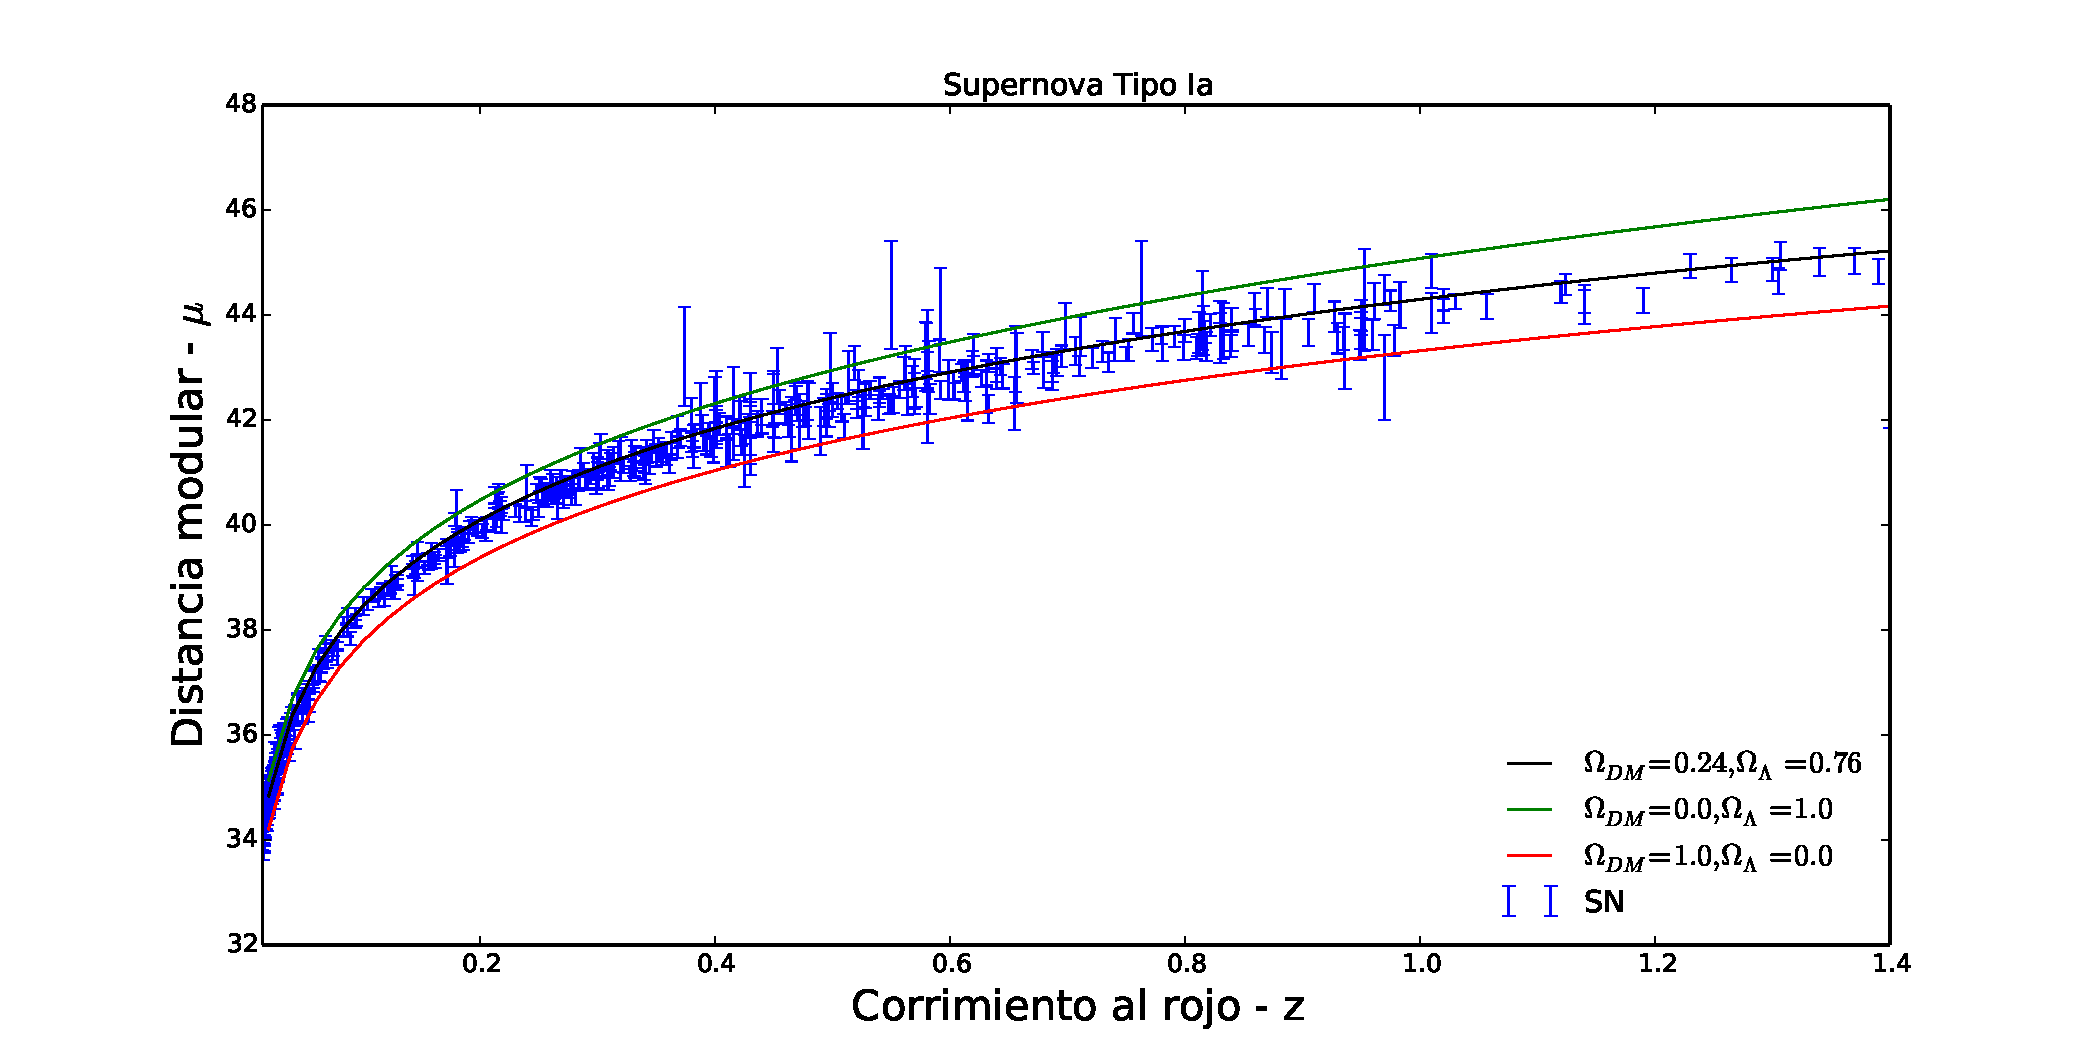
\includegraphics[trim =  0mm  0mm 0mm 0mm, clip, width=14cm, height=7cm]{SN_models.pdf} 
\end{center}
\caption[Geometries of the spacetime]
{Las l\'ineas s\'olidas representan los valores te\'oricos del m\'odulo de la distancia para tres modelos distintos,
mientras que los datos son obtenidos a partir de mediciones de Supernovas tipo Ia.}
\label{Fig:SNs}
\end{figure}


%%============================================================%%
\section{Estad\'istica Bayesiana}
%%============================================================%%



Durante la \'ultima d\'ecada la informaci\'on proveniente de un amplio rango de fuentes se ha incrementado sorprendentemente,
por ejemplo de la radiaci\'on c\'osmica del fondo de microondas, de Supernovas y de la estructura a gran escala del universo.
En este art\'iculo nos enfocaremos en traducir la informaci\'on experimental/observacional en constricciones de nuestros modelos 
resumido en la estimaci\'on de los par\'ametros cosmol\'ogicos involucrados.
Uno de los objetivos principales de la cosmolog\'ia observacional es determinar 
la combinaci\'on de par\'ametros que mejor describen los datos observacionales.
En esta secci\'on introduciremos brevemente los conceptos matem\'aticos b\'asicos 
necesarios para poder emplear el formalismo Bayesiano a la cosmolog\'ia. 
% Para esto enfocaremos nuestro an\'alisis 
%en la inferencia Bayesiana.
\\


%\section*{Estad\'istica Bayesiana vs Frecuentista}

%Antes de comenzar nuestra incursi\'on a trav\'es de la estad\'istica Bayesiana es importante conocer las 
%principales diferencias que distinguen un pensamiento Bayesiano de uno Frecuentista. 
%As\'i pues, en esta secci\'on introducieron estas discrepancias, analizando las consecuencias 
%desprendidas de estos conceptos.


%Posteriormente, 
%nos concentraremos en las herramientas computacionales que nos 
%ayudar\'an a simplificarnos la vida cuando un an\'alisis anal\'itico no sea posible (que ser\'a pr\'acticamente en todos los casos). 
%\\

Comenzaremos definiendo el concepto m\'as importante para cualquier procedimiento estad\'istico, 
esto es, el concepto de probabilidad. Si consideramos que $x$ es una variable aleatoria relacionada 
con un evento en particular y $P(x)$ su probabilidad correspondiente, entonces para ambos casos se debe cumplir que
%
	\begin{subequations}\label{axiomas}
		\begin{equation}\label{1a}
			P(x)\geq 0,
		\end{equation}
%		
		\begin{equation}\label{1b}
			\int_{-\infty}^\infty dxP(x) = 1,
		\end{equation}
%
y adem\'as para eventos mutuamente excluyentes,
%
		\begin{equation}\label{1c}
			P(x_1 \cup x_2) = P(x_1)+P(x_2), \ \ \ \ \text{si }x_1\cap x_2 = \emptyset.
		\end{equation}
%
En general
%
		\begin{equation}\label{1d}
			P(x_1,x_2) = P(x_1)P(x_1|x_2)
		\end{equation}
	\end{subequations}
%
La \'ultima regla nos dice que la probabilidad de que $x_1$ y $x_2$ ocurran estar\'a determinada por el 
producto de la probabilidad de que $x_1$ ocurra multiplicada por la probabilidad condicional de que $x_2$ 
ocurra tal que $x_1$ ha ocurrido tambi\'en.
\\

%Y entonces uno se preguntar\'ia en qu\'e consiste la diferencia entre la estad\'istica Bayesiana y la Frecuentista. 
%Y la respuesta radica principalmente en la definici\'on de probabilidad. 
%En la estad\'istica frecuentista, probabilidad est\'a fundamentalmente relacionada con una \textit{frecuencia de eventos}, 
%i.e. $p=n/N$, donde $n$ es el numero de sucesos de un evento, mientras que $N$ es el n\'umero total de intentos. 
%Por otro lado, en la estad\'istica Bayesiana, la probabilidad esta fundamentalmente 
%relacionada con el \textit{conocimiento que tenemos sobre alg\'un evento}.
%\\

Ahora bien, cualquier procedimiento estad\'istico  consiste de tres ingredientes b\'asicos que deben ser 
entendidos: 
%dependiendo el tipo de estad\'istica que estemos empleando:  
los datos, el modelo y un m\'etodo de estimaci\'on.

\begin{itemize}
\item \textit{Los datos}. Son una medida de nuestras observaciones, los cuales denotaremos como $D$. 
%Para un estad\'istico Frecuentista, dichos datos son el producto de un evento repetible, mientras 
%que para uno Bayesiano los datos se observan a partir de una muestra realizada, no necesariamente repetible, 
%por lo que estos deben tomarse fijos para el an\'alisis estad\'istico.

\item \textit{El modelo}. 
%Este concepto depende de la interpretaci\'on estad\'istica estemos utilizando. 
En general, un \textit{modelo} $Q$ es una colecci\'on de mediciones de probabilidades $P$. 
Las distribuciones $P_\theta$ son llamadas distribuciones del modelo, donde $\theta$ son aquellos 
par\'ametros que contiene $Q$. 
%La diferencia entre ambas clases de estad\'iticas recae en el valor 
%que los par\'ametros $\theta$ pueden tener. Mientras que para un pensamiento frecuentista los par\'ametros 
%$\theta$ son fijos y existe s\'olo un valor del par\'ametro $\theta_0$ al que nuestros datos pertenecen, 
%para un Bayesiano los par\'ametros $\theta$ no poseen un \'unico valor. De hecho, 
En la estad\'istica Bayesiana se considera que no existe diferencia matem\'atica formal entre par\'ametros 
y datos, por lo que para ambos casos se debe asociar una distribuci\'on de probabilidad.

\item Finalmente nos encontramos con el estimador de $P_0$. Un estimador para $P_0$ es la representaci\'on 
de nuestra ``mejor creencia" de $P$ dados los datos $D$, i.e. $P_0 = P_{mejor}$. 

\end{itemize}
%De esta manera en la tabla \ref{table:1} podemos resumir las principales diferencias entre ambas estad\'isticas. 


%\begin{table}[h!]
%\centering
%\begin{tabular}{c|c} 
% \hline
% \textbf{Frecuentista} & \textbf{Bayesiano} \\ [0.5ex] 
% \hline\hline
% Los datos son una muestra aleatoria  & Los datos son observados a partir de la    \\ 
% repetible. Existe una frecuencia de eventos. &muestra realizada. \\
% \hline 
%Los par\'ametros del modelo se mantienen& Los par\'ametros son desconocidos y deben ser \\
% constantes durante este proceso repetible. & descritos probabil\'isticamente. \\
%\hline
%Los par\'ametros se toman fijos. & Los datos se toman fijos.\\ [1ex] 
 %\hline
%\end{tabular}
%\caption{\footnotesize{Principales diferencias entre las interpretacion Frecuentista y la Bayesiana.}}
%\label{table:1}
%\end{table}

%\section{Introducci\'on a la Estad\'istica Bayesiana}



\subsection{Teorema de Bayes, priors, posteriores y esas cosas}

El tratamiento Bayesiano de un problema estad\'istico se centra en el  teorema de Bayes. 
Este teorema es una concecuencia directa de los axiomas de la probabilidad \eqref{axiomas}. 
Podemos observar de \eqref{1c}, sin p\'erdida de generalidad, que siempre es posible reescribir 
$P(x_2,x_1)=P(x_2)P(x_2|x_1)$. Luego, como es de esperarse que la relaci\'on $P(x_1,x_2)=P(x_2,x_1)$ se cumpla, 
obtenemos que

	\begin{equation}
		P(x_2|x_1)=\frac{P(x_2)P(x_1|x_2)}{P(x_1)}.
	\end{equation}
%
Este resultado es conocido como el \textit{teorema de Bayes}. Por otro lado, ya que 
%hab\'iamos  mencionado anteriormente que 
en la estad\'istica Bayesiana no existe distinci\'on formal entre datos y par\'ametros, 
podemos reescribir la ecuaci\'on anterior haciendo los cambios $x_1\rightarrow D$ y $x_2\rightarrow H$, como
%
	\begin{equation}\label{BayesT}
		P(\theta,H|D)=\frac{P(\theta,H)P(D|\theta,H)}{P(D)}
	\end{equation}

\noindent
En esta expresi\'on agregamos el t\'ermino $\theta$ para especificar que $H$ depende de dichos par\'ametros. 
Por otro lado, notemos que hemos agregado una nueva cantidad $H$, que llamaremos nuestra ``hip\'otesis". 
Esta \'ultima corresponde al modelo $Q$ que seg\'un nuestra creencia mejor se ajustar\'ia a los datos, i.e. $H=Q_{mejor}$.

Notemos, de la expresi\'on anterior, que contamos con cuatro nuevos entes que deben ser entendidos 
a la perfecci\'on.  En primera instancia $P(\theta,H|D)$ 
es conocida como la distribuci\'on posterior de probabilidad (o s\'implemente posterior). Esta cantidad es 
b\'asicamente el resultado principal a obtener ya que nos habla sobre la probabilidad de nuestro modelo 
(o par\'ametros del modelo). 
%tal que hemos obtenido cierto conjunto de datos $D$. 
Usualmente, dicha cantidad 
se utiliza para acotar los par\'ametros del modelo. Luego tenemos los denominados ``priors", $P(\theta,H)$, 
los cuales son una distribuci\'on de probabilidad para nuestros par\'ametros, definidos a partir de nuestro 
propio conocimiento acerca del modelo. Generalmente, en el l\'imite donde tenemos muchos datos, estos 
priors no son estad\'isticamente importantes, por lo que un prior t\'ipico para cada par\'ametro del 
modelo es uno plano (una distribuci\'on uniforme). A continuaci\'on tenemos lo que es conocido como el 
Likelihood $L(D;\theta)\equiv P(D|\theta,H)$ y es b\'asicamente el elemento m\'as importante al momento 
de hacer un estudio estad\'istico para la inferencia de los par\'ametros de nuestro modelo. Nos concentraremos 
en este elemento m\'as adelante. Finalmente nos encontramos con la evidencia Bayesiana (o s\'implemente evidencia). 
Podemos notar que \'esta act\'ua como un factor de normalizaci\'on

	\begin{equation}\label{BayesT2}
		P(D) = \int d\theta P(\theta,H)P(D|\theta,H).
	\end{equation}

\noindent
Esta cantidad es usualmente ignorada cuando el espacio de par\'ametros de un \'unico 
modelo es probado. Sin embargo resulta ser fundamental si lo que se quiere es hacer una 
comparaci\'on entre modelos. Para prop\'ositos de este art\'iculo omitiremos esta cantidad.

Podemos ver que el teorema de Bayes tiene una implicaci\'on enorme respecto a una inferencia 
(de par\'ametros, por ejemplo) desde el punto de vista Bayesiano. En un escenario t\'ipico podemos 
tomar un conjunto de datos y esperar interpretarlos en t\'erminos de alg\'un modelo. Sin embargo, 
lo que usualmente podemos hacer es lo opuesto, es decir, podemos tener un conjunto de datos y 
posteriormente confrontar un modelo tomando en cuenta la probabilidad que nuestro modelo se ajuste a los datos. 
De esta manera, como se puede ver de \eqref{BayesT}, el teorema de Bayes nos permite relacionar ambos 
escenarios, dandonos la posibilidad de conocer cual es el modelo (o par\'ametros del modelo) que mejor se ajusta a los datos.

\subsection{Likelihood}

Tomando el teorema de Bayes \eqref{BayesT}, pero por ahora ignorando la evidencia Bayesiana y considerando 
un prior uniforme, el c\'alculo de la probabilidad aposteriori esta determinado \'unicamente por maximizar el Likelihood. 
Por supuesto, el ignorar la evidencia ocasiona que no sea posible el poder dar una probabilidad absoluta 
de los par\'ametros de nuestro modelo, sin embargo, lo que s\'i podemos hacer es dar una probabilidad relativa 
definida como el cociente entre probabilidades. De esta manera, el Likelihood en un punto particular en el espacio 
de par\'ametros puede ser comparado con el que mejor se ajuste a las observaciones, $L_{max}$. Podemos decir 
entonces que un modelo es aceptable si el cociente de los Likelihoods

	\begin{equation}
		\Lambda=-2\ln\left[\frac{L(D;\theta,H)}{L_{max}}\right]
	\end{equation}
es mayor que alg\'un n\'umero dado.

Por otra parte, notemos que si nuestro posterior posee un \'unico m\'aximo global en $\theta_0$, 
siempre es posible hacer una expansi\'on en serie de la forma

	\begin{equation}
		\ln L(D;H)=\ln L(D;H_0)+\frac{1}{2}(\theta_\alpha-\theta_{0\alpha})\frac{\partial^2\ln L}
			{\partial\theta_\alpha \partial\theta_\beta}(\theta_\beta-\theta_{0\beta})+...
	\end{equation}

\noindent
donde $H_0$ corresponde al modelo con los par\'ametros que mejor se ajustan a los datos y 
$\theta_{0\alpha}$ son los componentes del vector de par\'ametros $\theta_0$.
De esta manera podemos reescribir nuestro Likelihood como
%	
	\begin{equation}\label{GLik}
		L(D;H)=L(D;H_0)\exp \left[-\frac{1}{2}(\theta_\alpha-\theta_{0\alpha})H_{\alpha\beta}(\theta_\beta-\theta_{0\beta})\right]
	\end{equation}
%
donde
%
%	\begin{equation}
$		H_{\alpha\beta}=\partial^2\ln L/ \partial\theta_\alpha \partial\theta_\beta$
%	\end{equation}
%
es llamada la matriz Hessiana y controla si la estimaci\'on de $\theta_\alpha$ y $\theta_\beta$ 
se encuentran correlacionadas. Si esta es diagonal, se dice que las estimaciones no est\'an correlacionadas.
%
Aqu\'i es preciso remarcar que la aproximaci\'on es buena siempre que contemos con un \'unico m\'aximo 
global en nuestro posterior. Si por el contrario \'este posee m\'ultiples m\'aximos locales, entonces la aproximaci\'on no servir\'ia.

%\subsection{Actualizando los posteriores}

%Una pregunta natural que puede surgir al momento de hacer cualquier an\'alisis Bayesiano es: ?`qu\'e pasa cuando obtengo nuevos datos? es decir, ?`puedo hacer uso de la informaci\'on que ya conoc\'ia o es preciso volver a calcular todo tomando como mi conjunto de datos los datos viejos m\'as los nuevos? Como [referencias] explica, siempre que los datos sean consistentes entre ellos, no importa cual sea la manera que se elija para analizar los datos, i.e. da lo mismo si primero se utilizan los datos viejos para obtener un posterior y luego dicho posterior se utiliza como prior para analizar los datos nuevos, que tomar el conjunto completo de datos y analizarlos con un prior inicial, digamos uno no informativo (plano).

\subsection{Chi-cuadrada}

Como se coment\'o anteriormente, la forma precisa para encontrar el posterior de alg\'un modelo en 
particular estar\'a dado por la maximizaci\'on  del Likelihood. Notemos que en la aproximaci\'on gaussiana, dicho 
tarea es equivalente a minimizar la expresi\'on 
%
	\begin{equation}\label{chi2}
		\chi^2\equiv(\theta_\alpha-\theta_{0\alpha})H_{\alpha\beta}(\theta_\beta-\theta_{0\beta}).
	\end{equation}

\noindent
La cantidad $\chi^2$, usualmente llamada \textit{chi-cuadrada}, se relaciona con el Likelihood 
Gaussiano v\'ia $L=L_0^{-\chi^2/2}$. As\'i pues, podemos decir que el proceso de maximizar un 
Likelihood Gaussiano es equivalente con el de minimizar un chi-cuadrada. 
%Sin embargo, en las 
%circunstancias donde un Likelihood no pueda ser bien especificado por una distribuci\'on gaussiana, 
%entonces ambos procesos ser\'an totalmente distintos.

\subsection{Curvas de contorno y regiones de confidencia}

Una vez que se han obtenido los par\'ametros que mejor se ajustan a los datos, lo que nos gustar\'ia saber 
es si hay regiones de confidencia donde otros par\'ametros pueden ser considerados como buenos candidatos 
para nuestro modelo. Una elecci\'on natural ser\'ia considerar regiones donde $\chi^2$ es menor que alg\'un 
cierto valor dado. Para el caso de distribuciones Gaussianas, como es el caso de \eqref{GLik}, 
dichas regiones corresponden con elipsoides.

\noindent
La forma en la que estas regiones de confidencia pueden ser calculadas es un poco t\'ecnica para los 
fines de este cap\'itulo, sin embargo, para los lectores interesados se les recomienda revisar las referencias [ref].

\subsection{Marginalizaci\'on}

Se puede dar el caso en el que al realizar un experimento s\'olo estemos interesados en analizar ciertos 
par\'ametros de nuestro modelo o existan par\'ametros extras considerados como ruido. Un ejemplo de 
estos par\'ametros de ruido podr\'ia ser aquellos correspondientes a efectos de calibraci\'on del experimento. 
Si este es el caso, lo que usualmente se hace es marginalizar sobre los par\'ametros que no son de inter\'es 
mediante la expresi\'on
%
	\begin{equation}
		P(\theta_1,...,\theta_j,H|D)=\int d\theta_{j+1}...d\theta_{m}P(\theta,H|D)
	\end{equation}
donde $m$ es el n\'umero total de par\'ametros en nuestro modelo y $\theta_1,...,\theta_j$ 
corresponden a los par\'ametros en los que estamos interesados.

\section{M\'etodos Num\'ericos}

En un escenario t\'ipico casi nunca es posible hacer el c\'alculo del posterior de manera anal\'itica. 
Para estas circunstancias existe toda una caja de herramientas computacionales que pueden 
ayudarnos a realizar esta tarea de forma num\'erica. En esta secci\'on nos enfocaremos en revisar 
las herramientas m\'as simples (pero no por eso menos eficientes) que est\'an a nuestra disposici\'on.

\subsection{MCMC para la inferencia de par\'ametros}

Una secuencia $X_1$, $X_2$, ... de elementos aleatorios se dice que es una cadena de Markov 
si la distribuci\'on condicional de $X_{n+1}$ dados $X_1,...,X_n$ depende \'unicamente de $X_n$. 
Lo que es importante de este proceso es que se puede demostrar que \'estas convergen a un estado 
estacionario donde varios elementos sucesivos de la cadena recaen. De esta manera, es posible estimar 
todas las cantidades de inter\'es, por ejemplo promedios, varianza, etc.. 

El uso de este m\'etodo en nuestro an\'alisis Bayesiano es el de tratar de muestrear nuestro 
posterior con ayuda de estas cadenas. Para esto $P(\theta,H|D)$ es aproximada por un conjunto de funciones delta
%
	\begin{equation}
		p(\theta,H|D)\simeq \frac{1}{N}\sum_{i=1}^N \delta(\theta-\theta_i)
	\end{equation}

\noindent
As\'i, el promedio de nuestro posterior puede ser calculado como 
%
	\begin{equation}
		\langle\theta\rangle=\int d\theta \theta P(\theta,H|D)\simeq \frac{1}{N}\sum_{i=1}^N\theta_i
	\end{equation}

\noindent
De esta manera, podemos promediar sobre funciones de nuestros par\'ametros mediante la expresi\'on 
%
	\begin{equation}
	\langle f(\theta)\rangle \simeq\frac{1}{N}\sum_{i=1}^N f(\theta_i)
	\end{equation}


\subsubsection{Algoritmo ``Metropolis Hasting"}

Como se explic\'o anteriormente, en un proceso MCMC es necesario proponer un nuevo 
paso en nuestra cadena tomando s\'olo como informaci\'on el paso presente. Sin embargo, 
como es de esperarse, necesitamos un criterio de aceptaci\'on (o rechazo) de este nuevo paso, 
dependiendo de si \'este resulta ser mejor para nuestro modelo o no. Por otro lado, si resulta 
que el nuevo paso es mejor, nos gustar\'ia no siempre aceptarlo, ya que de hacerlo se podr\'ia 
dar el caso de que no estemos mapeando completamente el espacio de par\'ametros e ir 
convergiendo a lo que podr\'ia ser un m\'aximo local de probabilidad para nuestro posterior. 
El algoritmo m\'as simple que contiene toda esta informaci\'on en su metodolog\'ia es conocido 
como el \textit{algoritmo de Metropolis Hasting} (MHA). \'Este b\'asicamente 
consiste en lo siguiente:

\noindent
 Comenzando con un punto inicial aleatorio $\theta_i$, con probabilidad 
posterior asociada $p_i = P(\theta_i,H|D)$, se necesita proponer un candidato $\theta_c$ tom\'andolo 
de alguna \textit{distribuci\'on propuesta} $q(\theta_i,\theta_c)$ que sea sim\'etrica, i.e. $q(\theta_i,\theta_c)=
q(\theta_c,\theta_i)$. De esta manera, la probabilidad de aceptar un nuevo punto estar\'ia dada por 
%
	\begin{equation}
		p(aceptar)=min\left[1,\frac{p_c}{p_i}\right]
	\end{equation}

As\'i, el algoritmo completo puede ser descrito por los siguientes pasos:
%
	\begin{enumerate}
		\item Elegir un valor inicial aleatorio $\theta_i$ en el espacio de par\'ametros y calcular su correspondiente posterior.
		\item Generar un nuevo candidato en el espacio de par\'ametros considerando alguna distribuci\'on propuesta 
			y calcular su 	correspondiente posterior.
		\item Aceptar (o no) el nuevo punto con ayuda del MHA.
		\item Si el punto no es aceptado, repeterir el punto anterior en la cadena.
		\item Repetir los pasos del 2 al 4 hasta tener una cadena lo suficientemente larga.
	\end{enumerate}

\subsection{Pruebas de convergencia}

Es clara la necesidad de alg\'un criterio que nos permita saber cuando nuestras cadenas 
han convergido al estado estacionario, de lo contrario, uno podr\'ia tener una gran p\'erdida de 
tiempo computacionalmente hablando. La forma m\'as simple de 
hacer dicha prueba consiste en correr multiples cadenas y detectar a simple vista  
que todas converjan a la misma regi\'on de par\'ametros. Sin embargo, existen m\'etodos m\'as formales 
que nos permiten hacer dicha verificaci\'on. La prueba cl\'asica de convergencia utilizada en Cosmolog\'ia 
es el llamado \textit{criterio de convergencia de Gelman-Rubin}  (1992) \cite{AlanH,LicV2}. En \'este se considera que una 
cadena ha convergido siempre que la cantidad 
%
	\begin{equation}
		\hat R=\frac{\frac{N-1}{N}W+B(1+\frac{1}{M})}{W},
	\end{equation}

\noindent
se aproxime a la unidad. Un criterio t\'ipico de convergencia es cuando $R<1.03$. En esta expresi\'on $M$ 
es el n\'umero total de cadenas, $N$ el n\'umero de puntos por cadena, $B$ es la varianza relacionada entre cadenas y
$W$ es la varianza de cada cadena. 
% 
	\begin{equation}
		B=\frac{1}{M-1}\sum_{j=1}^M(\langle\theta^j\rangle-\langle\theta\rangle)^2, \qquad 
				W=\frac{1}{M(N-1)}\sum_{i=1}^N\sum_{j=1}^M(\theta_i^j-\langle\theta^j\rangle)^2
	\end{equation}



\subsection{Algunos detalles imporantes}

\textit{Sobre la distribuci\'on propuesta.-} La elecci\'on de una funci\'on propuesta para generar el 
nuevo paso en nuestra cadena es de vital importancia para la eficiencia al momento de hacer la 
inferencia en cuesti\'on. Se puede dar el caso de que si el paso propuesto en la funci\'on es 
muy peque\~no, entonces nuestro c\'odigo muestrear\'a muy lentamente el espacio de par\'ametros, 
lo que ocasionar\'ia que nuestro m\'etodo se hiciera muy ineficiente. Por otro lado, si el paso de 
nuestra funci\'on propuesta es muy grande ocasionar\'ia que este pudiera mapear de forma muy 
ineficiente el espacio de par\'ametros, haciendo saltos grandes y dejando el valor de nuestros 
par\'ametros que mejor se ajustan a los datos entre las regiones intermedias entre pasos.
\\ $ $ 

%\textit{Sobre el ``burn-in"}.- Dado que al generar nuestras cadenas solemos comenzar en un punto arbitrario del espacio de par\'ametros, existir\'an algunos puntos al inicio que no tendr\'an nada que ver con la regi\'on de par\'ametros que son de nuestro inter\'es. A estos puntos iniciales es a lo que se le denomina el \textit{``burn-in"} de la cadena y debe ser ignorada durante el an\'alisis estad\'istico.
%\\ $ $ \\

%\textit{Pruebas de autocorrelaci\'on.-} Una forma complementaria de ver por convergencia en una estimaci\'on utilizando MCMCs es viendo la autocorrelaci\'on entre las muestras. La autocorrelaci\'on $\log k$ es definida como la correlaci\'on entre todas las muestras y la muestra $k$. \'Esta puede ser cuantificada por calcular [ref]
%\begin{equation}
%\rho_k=\frac{Cov(X_t,X_{t+k})}{\sqrt{Var(X_t)Var(X_{t+k})}}=\frac{E[(X_t-X)(X_{t+k}-X)]}{\sqrt{E[(X_t-X)^2]E[(X_{t+k}-X)^2]}}
%\end{equation}
%donde $X_i$ es la i-\'esima muestra y $X$ es el promedio de las muestras. Esta autocorrelaci\'on debe hacerse peque\~na conforme $k$ crece, lo que implicar\'ia que las muestras comienzan a ser independientes.

\section{Ajustando una l\'inea recta}

En esta secci\'on pondremos en uso las herramientas aprendidas anteriormente con uno de los 
ejemplos m\'as simples que hay: ajustar una l\'inea recta. Para esto, primero generaremos un 
conjunto de 25 datos a lo largo de la recta $y=1+x$. Digamos que estos datos fueron obtenidos 
a partir de una teor\'ia en que la l\'inea recta es el modelo que puede describir al sistema. 
Para dificultar un poco m\'as las cosas, vamos a agregar a cada dato un ruido gaussiano con 
desviaci\'on estandar $\sigma = 0.3$, que puede ser debido a problemas en la medici\'on. 
Con esto, nuestros datos lucir\'an como se pueden ver en la figura \ref{dat}.


\begin{figure}[ht] 
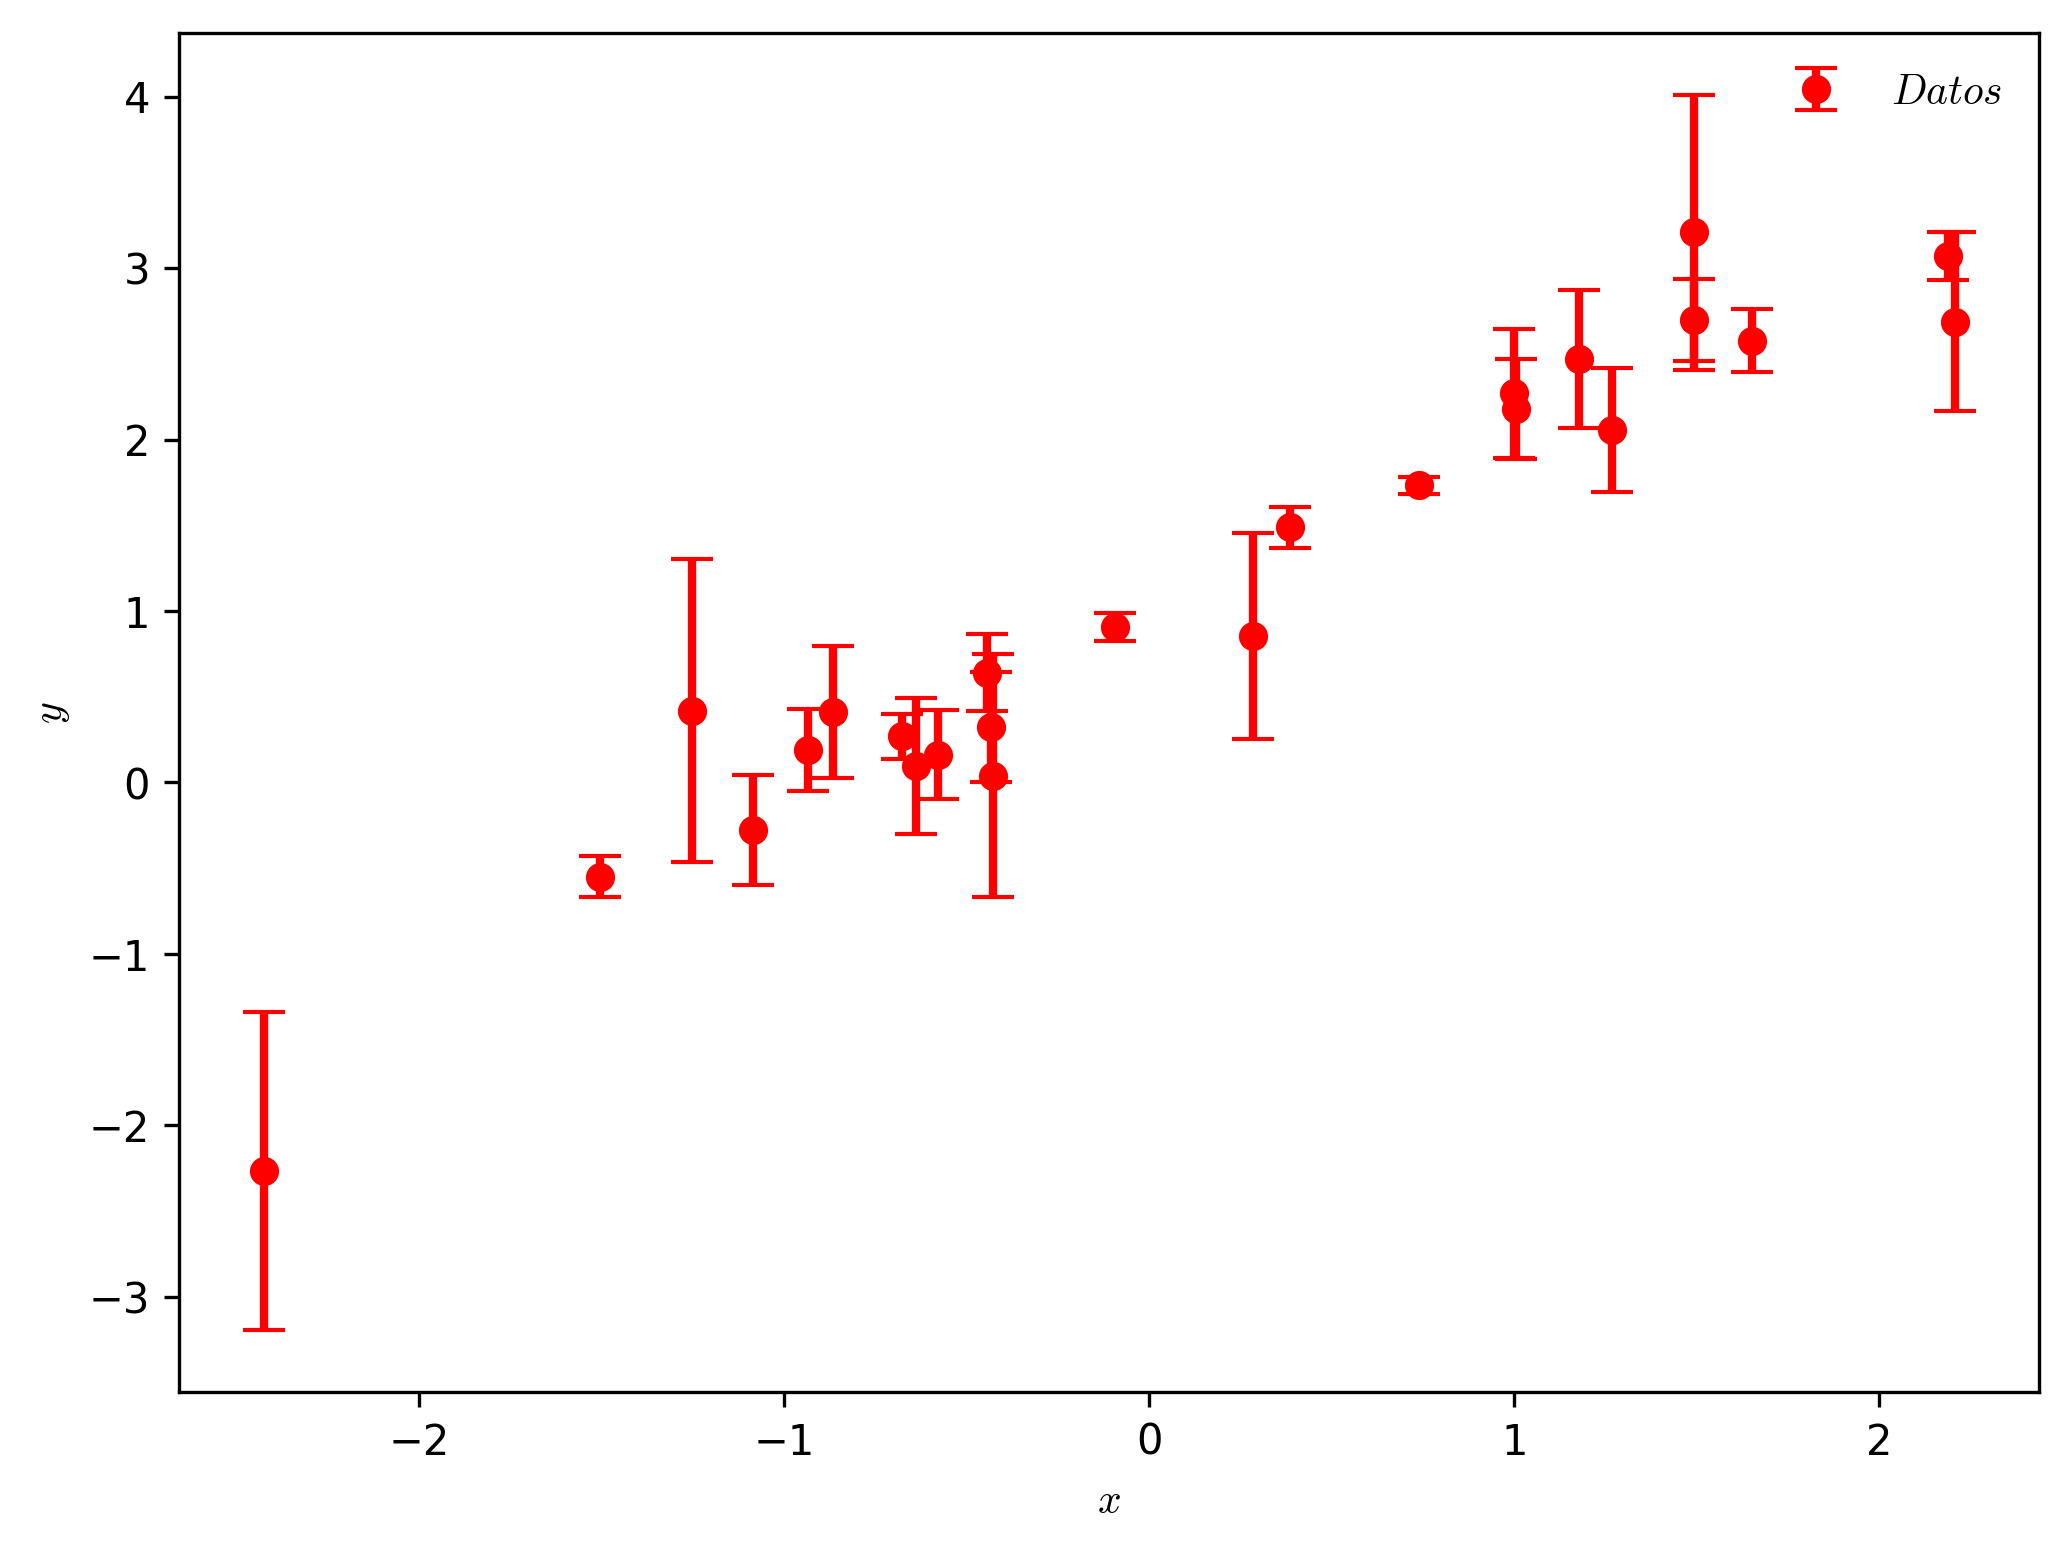
\includegraphics[trim = 1mm  1mm 1mm 1mm, clip, width=8.cm, height=5cm]{data.png}
\caption{Datos a lo largo 
de la recta $y=1+x$ con un ruido gaussiano con desviaci\'on estandar $\sigma = 0.3$.}% \citep{LiddleLyth}.}
\label{dat}
\end{figure}


Ahora bien, supongamos que estamos interesados en conocer el valor de los par\'ametros 
$a$ y $b$ de nuestra recta $y=a+bx$, por lo que nos gustar\'ia estimar dichos par\'ametros 
mediante un proceso de inferencia Bayesiana. Si consideramos que en principio no conocemos nada sobre el valor de 
nuestros par\'ametros libres, salvo las cotas l\'imite en que \'estos deber\'ian estar, un buen prior para 
comenzar nuestra inferencia Bayesiana ser\'ia el considerar distribuciones planas. Para esto comenzaremos considerando los priors
%
	$
		a \propto U[0,1.5],  \text{y}  b \propto U[0,1.5].
	$
\\
Considerando que existen valores de $a$, $b$ y $\sigma$ para los cuales los datos se fijan mejor 
(tal que el posterior es m\'aximo global), entonces de \eqref{GLik} podemos escribir el Likelihood de nuestro sistema como 
%
	\begin{equation}
		L(D;recta)\propto \exp\left[-\frac{(y_d-y)^2}{2\sigma_d}\right].
	\end{equation}
donde $y_d$ son nuestros datos y $\sigma_d$ los errores estimados de nuestras mediciones.

Con esto ya podemos generar nuestras MCMC utilizando el MHA. Para \'esto hicimos uso del 
m\'odulo PyMC3 \cite{PyMC3} ya implementado en Python que nos permite emplear este m\'etodo de forma m\'as sencilla. 
Para el lector interesado, el c\'odigo puede encontrarse en \cite{Github}. En nuestro an\'alisis corrimos un total de 
6 cadenas con 10,000 pasos cada una. Nuestro resultado obtenido puede verse en la tabla \ref{tabla1} y la 
figura \ref{fig:chains}. Como podemos ver en el lado izquierdo de la figura, existen regiones para las cuales 
la frecuencia de eventos en nuestro muestreo se ve incrementada. De esta manera, podemos decir que 
dichas regiones poseen un posterior m\'as probable para ajustarse a nuestros datos. De hecho, de la 
tabla \ref{tabla1} podemos observar que los valores reales para $a$ y $b$ parecen encuentrarse dentro 
de una desviaci\'on est\'andar del valor promedio estimado para estos par\'ametros. Adicionalmente se obtuvo el valor del criterio 
de convergencia de Gelman-Rubin  para cada variable con la intenci\'on de verificar que nuestros resultados 
obtenidos han convergido. Como podemos ver este n\'umero es muy cercano a la unidad, por lo que nuestro 
criterio de convergencia se cumple.
%
\begin{table}[t!]
\centering
\begin{tabular}{||l|l|l|l||} 
 \hline
 & \textbf{Promedio} & \textbf{Desv. Est.} & \textbf{Gelman-Rubin} \\ [0.5ex] 
 \hline\hline
$a$ & 0.99057 & 0.034329 & 1.00029 \\
\hline
$b$ & 1.00467 & 0.03591 & 1.00026\\
\hline
\end{tabular}
\caption{\footnotesize{Promedios obtenidos tras nuestra inferencia Bayesiana. Se calcula tambi\'en el 
criterio de Gelman-Rubin para la convergencia de las cadenas.}}
\label{tabla1}
\end{table}

%Como se mencion\'o, tambi\'en es importante checar si no existe autocorrelaci\'on entre las 
%cadenas mediante las pruebas de autocorrelaci\'on. Como se puede observar en la figura \ref{autocorrplots}, 
%conforme $lag\ k$ crece, la correlaci\'on tiende a cero, lo que nos dice que en nuestras 
%muestras son independientes, con lo que podemos considerar que nuestro an\'alisis va bien y ha convergido completamente. 

\begin{figure}[ht] 
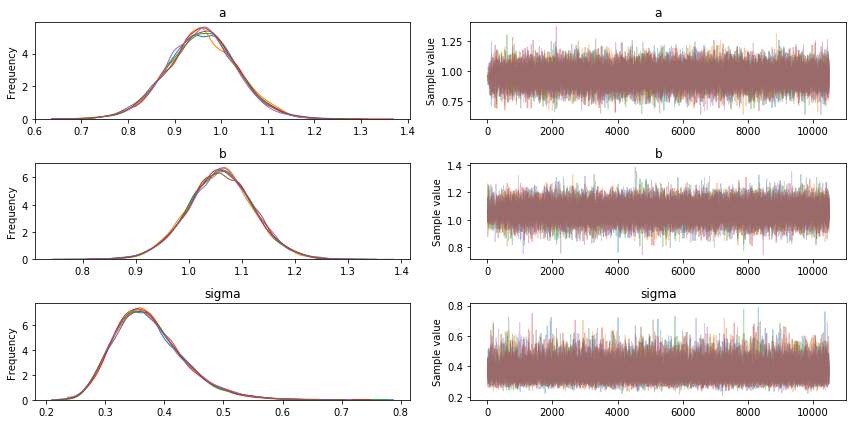
\includegraphics[trim = 1mm  1mm 1mm 1mm, clip, width=14.cm, height=5cm]{chain.png}
\caption{Resultados obtenidos de nuestro muestreo de pasos en nuestras cadenas de Markov}% \citep{LiddleLyth}.}
\label{fig:chains}
\end{figure}

Para ejemplificar los resultados obtenidos mediante este m\'etodo, podemos graficar la recta te\'orica considerando los valores promediados de nuestros par\'ametros proporcionados en la tabla \ref{tabla1}. En la figura \ref{fig:datastr} podemos observar esta gr\'afica. Como podemos observar, a pesar de que nuestra curva inferida por nuestro m\'etodo Bayesiano no coincide exactamente con la recta real, \'esta parece ajustar bastante bien nuestros datos. Por supuesto, esto se debe al hecho de que al contar con tan pocos datos, a\'un hay cierta ambig\"uedad en los par\'ametros que pueden ajustar relativamente bien a los datos. 

\begin{figure}[ht] 
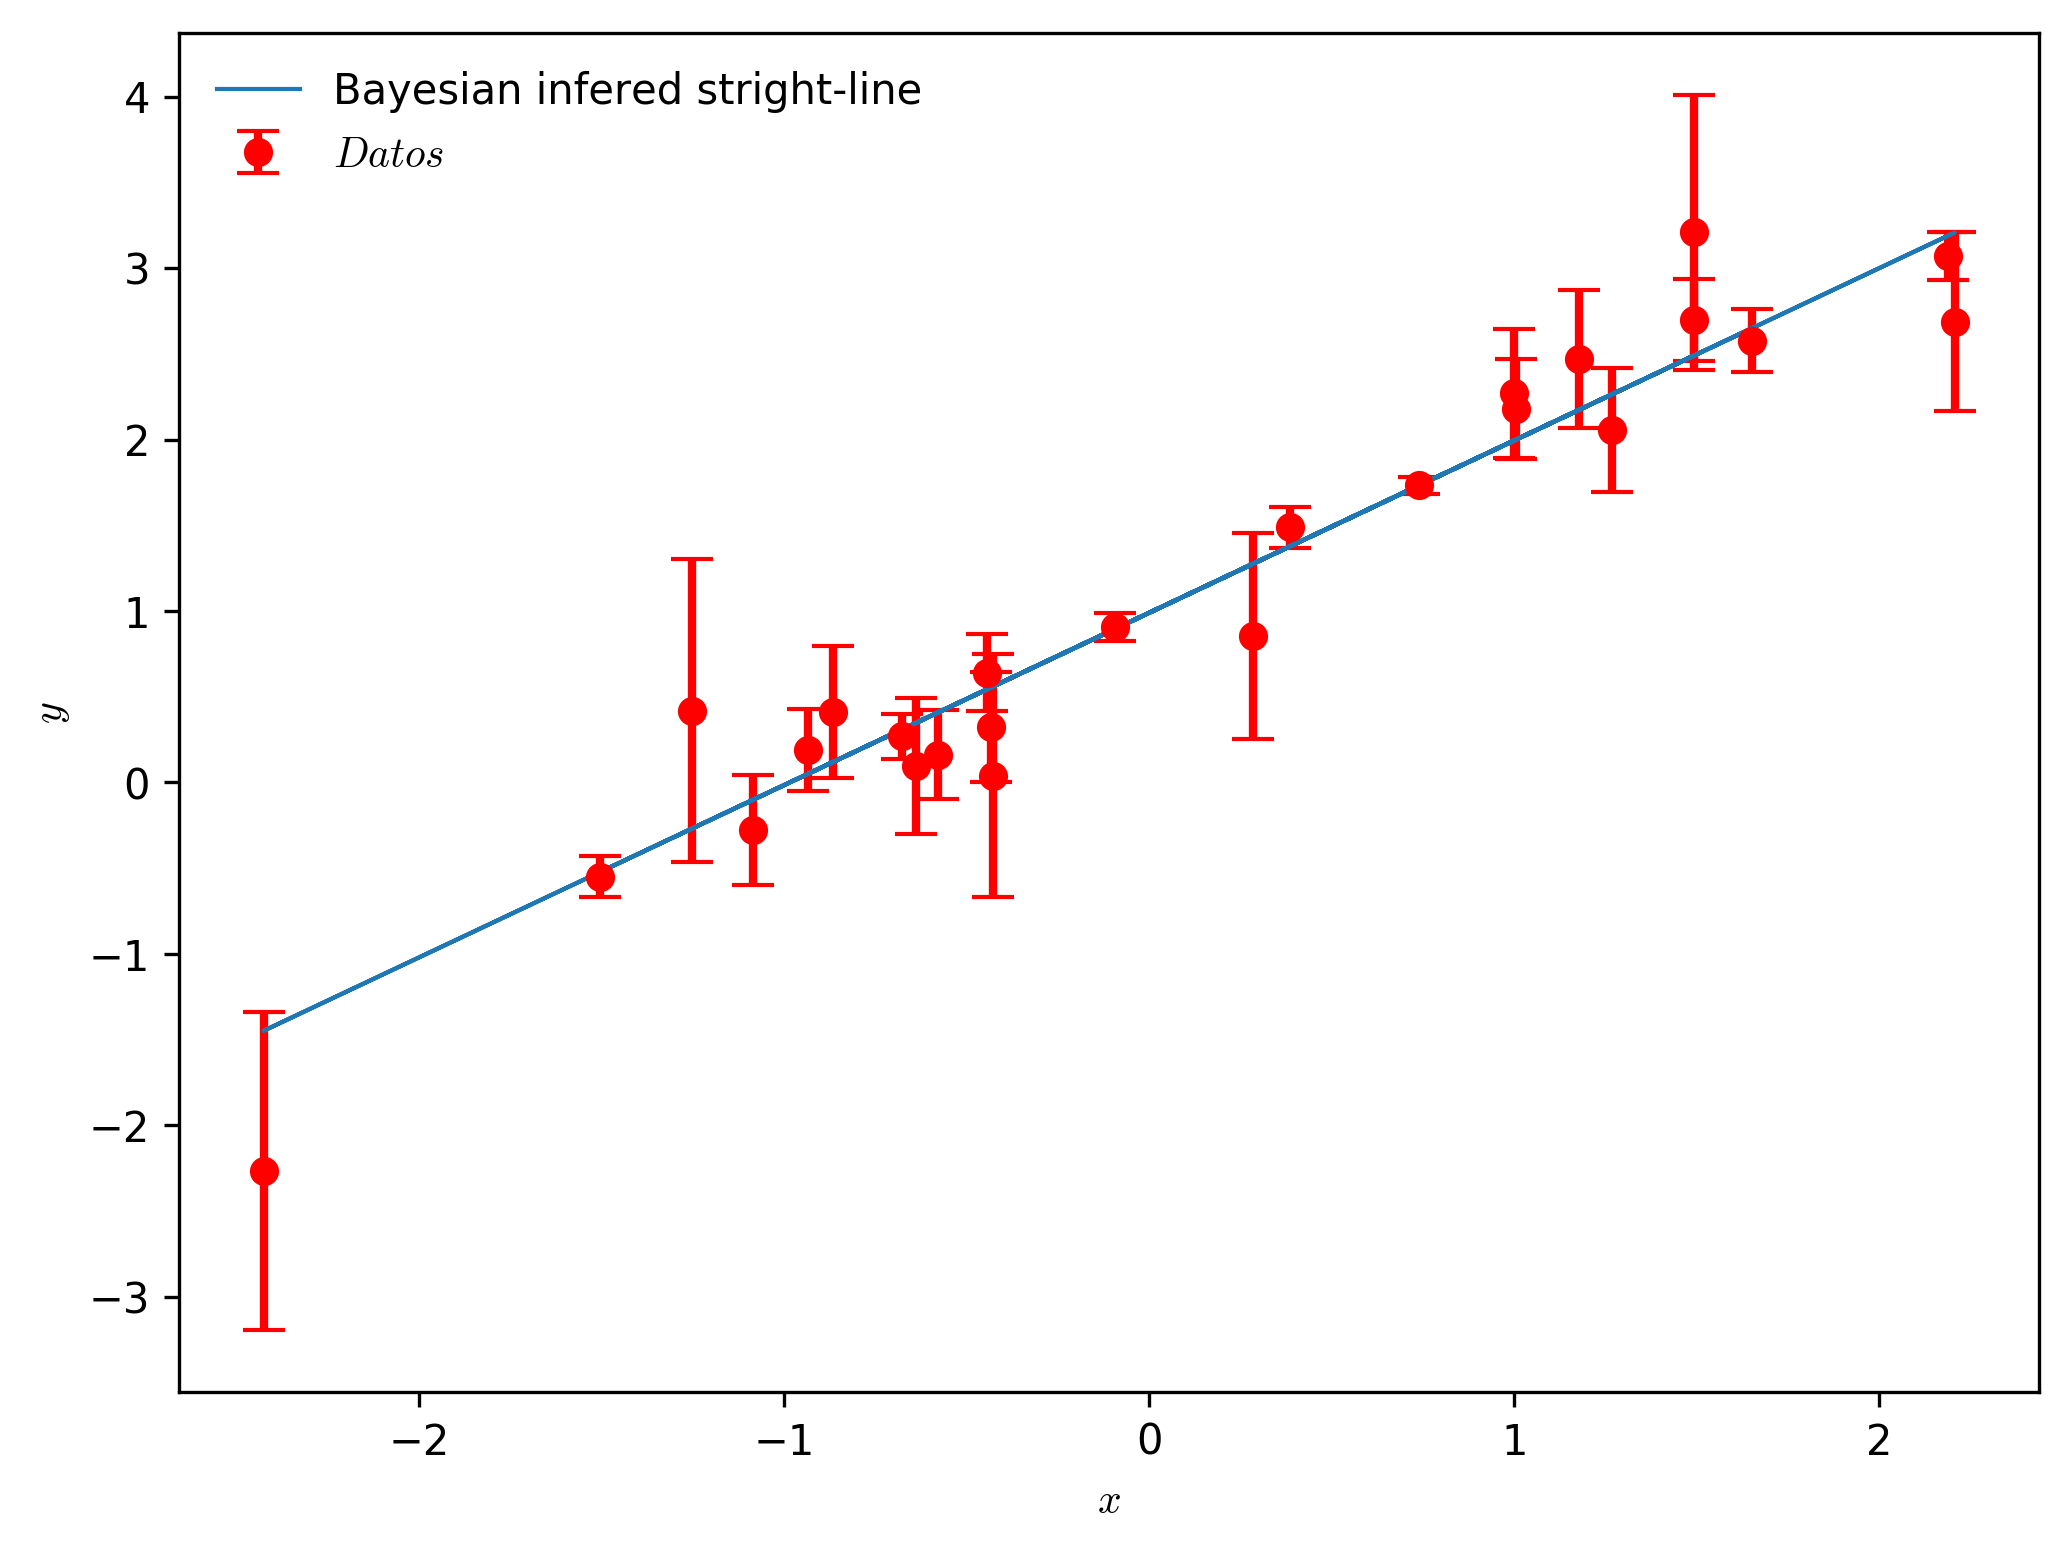
\includegraphics[trim = 1mm  1mm 1mm 1mm, clip, width=8.cm, height=5cm]{datastr.png} \qquad
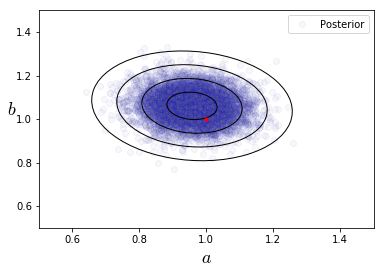
\includegraphics[trim = 1mm  1mm 1mm 1mm, clip, width=6.cm, height=5cm]{cab.png}
\caption{Derecha:Curva inferida por nuestro m\'etodo Bayesiano. Los par\'ametros obtenidos parecen ajustar muy bien nuestros datos.
Izquierda:Regiones de confidencia en 2D para nuestros par\'ametros $a$ y $b$. Graficamos los contornos a 1-4 $\sigma$. }% \citep{LiddleLyth}.}
\label{fig:datastr}
\end{figure}


%\begin{minipage}{\textwidth}
%\centering
%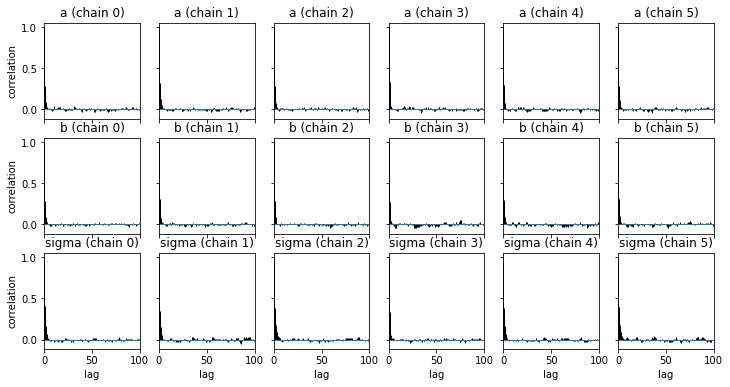
\includegraphics[height=8cm]{autocorrplots.png}
%\captionof{figure}{\footnotesize{Pruebas de autocorrelaci\'on.}}
%\label{autocorrplots}
%\end{minipage}
%\\ $ $

Finalmente s\'olo resta mostrar las t\'ipicas regiones de confidencia para nuestros par\'ametros. Las regiones que son usuales mostrar son aquellas que corresponden a un m\'ultiplo de desviaciones estandar de los par\'ametros de inter\'es. En la figura \ref{confidence} mostramos las t\'ipicas regiones de confidencia a 1-4 $\sigma$. Adem\'as hemos graficado en color rojo el valor real para nuestros par\'ametros. Lo que podemos observar r\'apidamente es que el valor real de nuestros par\'ametros se encuentran a menos de una desviaci\'on estandar del valor estimado por nuestro m\'etodo de inferencia. Por supuesto, la raz\'on de esta discrepancia es debido a que s\'olo contamos con 25 datos para hacer nuestra inferencia Bayesiana; de contar con m\'as, nuestros resultados deber\'ian ser m\'as precisos y podr\'iamos ser capaces de acotar en una regi\'on muy peque\~na los posibles valores que nuestros par\'ametros podr\'ian tener.  

%%%%%%%%%%%%%%%%%%%%%%%%%%%%%%%%%%%%%%%%%%%

\section{Estad\'istica Bayesiana con Supernovas}

%%%%%%%%%%%%%%%%%%%%%%%%%%%%%%%%%%%%%%%%%%%


%%%FIGURE
\begin{figure}[h]
\begin{center}
\includegraphics[trim =  0mm  0mm 0mm 0mm, clip, width=8cm, height=5cm]{constraints.pdf} 
\includegraphics[trim =  0mm  0mm 0mm 0mm, clip, width=8cm, height=5cm]{constraints_1.pdf} 
\end{center}
\caption[Geometries of the spacetime]
{A summary of possible geometries.}
\label{Fig:cmb_sh}
\end{figure}
%%%%%%%

Los resultados obtenidos utilizando SN $\Omega_{DM} =0.30 \pm 0.04, \Omega_b h^2 = 0.0224 \pm 0.0004, h = H_0/100 = 0.68 \pm 0.04
\Omega_k = -0.002 \pm 0.010$, y usando BAO 
$\Omega_{DM} = 0.301 \pm 0.008,   \Omega_b h^2 = 0.0225 \pm 0.0003,  h = H_0/100 = 0.679 \pm 0.007, 
\Omega_k = -0.003 \pm 0.003$ donde el error representa 68\% nivel de confianza.

\bibliography{cosmo,cosmo_preprints}

Once we have learned how to use a Bayesian procedure to fit a model, we can use this new tecniques in our Cosmological models. 



%\jav{tomando los parametros que mejor ajustan, graficar la linea teoria en la misma figura 2, tambien falta decir que 
%valor en el promedio $\pm$ su barra de error para a,b, m}

\bibliography{cosmo,cosmo_preprints}
%\bibitem{AlanH}{Alan Heaven} Alan Heavens; Statistical techniques in cosmology; May 2010
%\bibitem{LicV2} Verde L., astroph/0712.3028 (2007)
%\bibitem{PyMC3}Salvatier J., Wiecki T.V., Fonnesbeck C. (2016) Probabilistic programming in Python using PyMC3. PeerJ Computer Science 2:e55 DOI: 10.7717/peerj-cs.55.
%\bibitem{Github} https://github.com/LuisPaAl/Statistical-memories

\end{document}


